%%%%%%%%%%%%%%%%%%%%%%%%%%%%%%%%%%%%%%%%%%%%%%%%%%%%%%%%%%%%
\documentclass[a4paper,11pt,oneside]{article}
\usepackage[a4paper,vmargin={1.5cm,1.5cm},width=17cm]{geometry}
\usepackage[style=verbose-inote,doi=false,sortcites=true,block=space]{biblatex}
\usepackage[utf8]{inputenc}
\usepackage{textcomp}
\usepackage[spanish]{babel}
\usepackage{microtype}
\usepackage{lmodern}
\usepackage{graphicx}
\usepackage{fancyhdr}
\usepackage{booktabs}
\usepackage{eurosym}
\usepackage{hyperref}

%%%%%%%%%%%%%%%%%%%%%%%%%%%%%%%%%%%%%%%%%%%%%%%%%%%%%%%%%%%%
%% HEADERS
\setlength{\headheight}{1cm}
\setlength{\headsep}{0.5cm}
\pagestyle{fancyplain}
\fancyhf{}
\lhead{\fancyplain{}{\sc Memoria científico técnica de proyectos coordinados}}
\rhead{\fancyplain{}{\sc NEXT}}
\cfoot{\thepage}
\renewcommand{\headrulewidth}{0pt} % remove lines
\renewcommand{\footrulewidth}{0pt}

%%%%%%%%%%%%%%%%%%%%%%%%%%%%%%%%%%%%%%%%%%%%%%%%%%%%%%%%%%%%
%% Hack to make math formulas bold in section titles
\makeatletter
\DeclareRobustCommand*{\bfseries}{%
  \not@math@alphabet\bfseries\mathbf
  \fontseries\bfdefault\selectfont
  \boldmath
}
\makeatother

%%%%%%%%%%%%%%%%%%%%%%%%%%%%%%%%%%%%%%%%%%%%%%%%%%%%%%%%%%%%
\def\thesection{\bf \textsf{\alph{section}}}

%\nobibliography{biblio}
%\bibliographystyle{JHEP}

\bibliography{biblio}


%%%%%%%%%%%%%%%%%%%%%%%%%%%%%%%%%%%%%%%%%%%%%%%%%%%%%%%%%%%%
\begin{document}

%% Some useful definitions
% BB
\newcommand{\bb}{\ensuremath{\beta\beta}}
% BB0NU
\newcommand{\bbonu}{\ensuremath{\beta\beta0\nu}}
% BB2NU
\newcommand{\bbtnu}{\ensuremath{\beta\beta2\nu}}
% NME
\newcommand{\Monu}{\ensuremath{\Big|M_{0\nu}\Big|}}
\newcommand{\Mtnu}{\ensuremath{\Big|M_{2\nu}\Big|}}
% PHASE-SPACE FACTOR
\newcommand{\Gonu}{\ensuremath{G_{0\nu}(\Qbb, Z)}}
\newcommand{\Gtnu}{\ensuremath{G_{2\nu}(\Qbb, Z)}}

% mbb
\newcommand{\mbb}{\ensuremath{m_{\beta\beta}}}
\newcommand{\kgy}{\ensuremath{\rm kg \cdot y}}
\newcommand{\ckky}{\ensuremath{\rm counts/(keV \cdot kg \cdot y)}}
\newcommand{\mbba}{\ensuremath{m_{\beta\beta}^a}}
\newcommand{\mbbb}{\ensuremath{m_{\beta\beta}^b}}
\newcommand{\mbbt}{\ensuremath{m_{\beta\beta}^t}}
\newcommand{\nbb}{\ensuremath{N_{\beta\beta^{0\nu}}}}

% Qbb
\newcommand{\Qbb}{\ensuremath{Q_{\beta\beta}}}

% Tonu
\newcommand{\Tonu}{\ensuremath{T_{1/2}^{0\nu}}}

% Tonu
\newcommand{\Ttnu}{\ensuremath{T_{1/2}^{2\nu}}}

% Xe-136
\newcommand{\Xe}{\ensuremath{^{136}}Xe}

% Xe-136
\newcommand{\CS}{\ensuremath{^{137}}Cs}

% Xe-136
\newcommand{\NA}{\ensuremath{^{22}}Na}


% Bi-214
\newcommand{\Bi}{\ensuremath{^{214}}Bi}

% Tl-208
\newcommand{\Tl}{\ensuremath{^{208}}Tl}

% Pb-208
\newcommand{\Pb}{\ensuremath{^{208}}Pb}
% Pb-208
\newcommand{\PBD}{\ensuremath{^{210}}Pb}

% Po-214
\newcommand{\Po}{\ensuremath{^{214}}Po}

% bru
\newcommand{\bru}{cts/(keV$\cdot$kg$\cdot$y)}

% Saltos de carro en tablas
\newcommand{\minitab}[2][l]{\begin{tabular}{#1}#2\end{tabular}}

\newcommand{\thedraft}{0.1.1}% version for referees

\newcommand{\MO}{\ensuremath{{}^{100}{\rm Mo}}}
\newcommand{\SE}{\ensuremath{{}^{82}{\rm Se}}}
\newcommand{\ZR}{\ensuremath{{}^{96}{\rm Zr}}}
\newcommand{\KR}{\ensuremath{{}^{82}{\rm Kr}}}
\newcommand{\ND}{\ensuremath{{}^{150}{\rm Nd}}}
\newcommand{\XE}{\ensuremath{{}^{136}\rm Xe}}
\newcommand{\GE}{\ensuremath{{}^{76}\rm Ge}}
\newcommand{\GES}{\ensuremath{{}^{68}\rm Ge}}
\newcommand{\TE}{\ensuremath{{}^{128}\rm Te}}
\newcommand{\TEX}{\ensuremath{{}^{130}\rm Te}}
\newcommand{\TL}{\ensuremath{{}^{208}\rm{Tl}}}
\newcommand{\CA}{\ensuremath{{}^{48}\rm Ca}}
\newcommand{\CO}{\ensuremath{{}^{60}\rm Co}}
\newcommand{\PO}{\ensuremath{{}^{214\rm Po}}}
\newcommand{\U}{\ensuremath{{}^{235}\rm U}}
\newcommand{\CT}{\ensuremath{{}^{10}\rm C}}
\newcommand{\BE}{\ensuremath{{}^{11}\rm Be}}
\newcommand{\BO}{\ensuremath{{}^{8}\rm Be}}
\newcommand{\UDTO}{\ensuremath{{}^{238}\rm U}}
\newcommand{\CD}{\ensuremath{^{116}{\rm Cd}}}
\newcommand{\THO}{\ensuremath{{}^{232}{\rm Th}}}
\newcommand{\BI}{\ensuremath{{}^{214}}Bi}


%% Heading
\begin{center}
{\Large \textsf{Convocatorias 2014}} \\ \vspace{0.3cm}
{\Large  \textsf{Proyectos de I+D ``Excelencia'' y Proyectos de I+D+I ``Retos Investigación"}} \\ 
{\Large \textsf{Dirección General de Investigación Científica y Técnica}} \\
{\Large \textsf{Subdirección General de Proyectos de Investigación }} \\ 
%\vspace{0.5cm}
%{\LARGE \bf \textsf{Construcción puesta a punto y operación del experimento NEXT en el Laboratorio Subterráneo de Canfranc} }\\ 
%\vspace{0.3cm}
%{\LARGE \bf \textsf{Construction, commissioning and operation of the NEXT experiment at the Canfranc Underground Laboratory }}\\ 
\end{center}


\section{\bf \textsf{RESUMEN DE LA PROPUESTA/SUMMARY OF THE PROPOSAL}}
\subsection{\sc DATOS DEL PROYECTO COORDINADO}

{\sc INVESTIGADOR COORDINADOR PRINCIPAL:} Juan José Gómez Cadenas.
\vspace{0.3cm}

{\sc TÍTULO GENERAL DEL PROYECTO COORDINADO:} Construcción puesta a punto y operación del experimento NEXT en el Laboratorio Subterráneo de Canfranc.
\vspace{0.3cm}

{\sc ACRÓNIMO DEL PROYECTO COORDINADO:} NEXT.
\vspace{0.3cm}

{\bf RESUMEN DEL PROYECTO COORDINADO:} 
\vspace{0.3cm}

NEXT (Neutrino Experiment with a Xenon TPC) es un experimento para buscar desintegraciones doble beta sin neutrinos (\bbonu) utilizando cien kilos de gas xenón, enriquecido al 90\% en el isótopo \XE. La detección de dichos procesos demostraría unívocamente que el neutrino es una partícula de Majorana (es decir su propia antipartícula) y supondría un descubrimiento de suma importancia en física de partículas y cosmología. 

El experimento NEXT requiere la construcción de una serie de cámaras de proyección temporal (HPXe-TPC de sus siglas en inglés), que operan a alta presión (10-20 atmósferas) 
Sus características principales son: a) excelente resolución en la medida de la energía; b) capacidad de reconstruir la trayectoria de los electrones emitidos en la desintegración, una característica única de esta tecnología, que refuerza la capacidad del experimento para reducir el ruido de fondo; c) economía de escala, esto es la capacidad de mejorar el cociente señal a ruido a medida que el tamaño del detector aumenta; y d) la posibilidad de reducir el ruido de fondo hasta niveles despreciables mediante la técnica conocida como {\sc BaTa} (de las siglas en inglés, Barium Tagging).

NEXT es  una colaboración internacional, liderada por grupos españoles y con una fuerte contribución de grupos norteamericanos. El proyecto ha finalizado la fase de R\&D que se ha extendido desde 2009 hasta 2013. Durante esta fase se han construido los prototipos NEXT-DEMO (IFIC) y NEXT-DBDM (Berkeley) que han demostrado de manera rotunda las características principales de NEXT, incluyendo una excelente resolución en energía (0.5-0.7 \% FWHM a 2.5 MeV) y la reconstrucción de electrones. 

En el año 2014 se está construyendo la primera fase del experimento. Se trata de un detector capaz de albergar 15 kg de gas xenón, denominado NEXT-WHITE (NEW). La financiación para la construcción de NEW proviene de un Advanced Grant (AdG) concedido por la ERC al spokesperson de NEXT y IP de este proyecto coordinado. NEW tiene un tiple objetivo: a) certificación de la tecnología de NEXT en condiciones de radio-pureza extrema ; b) medida precisa de los ruidos de fondo en el experimento; y c) medida del proceso de desintegración doble beta estándar (\bbtnu). NEW será instalado en el Laboratorio Subterráneo de Canfranc (LSC) en 2015 y operará durante 2015 y 2016.

La siguiente fase del experimento es la construcción, puesta a punto y operación del detector NEXT-100, que albergará cien kilos de xenón (enriquecido al 90\% en \XE) a una presión de 15 atmósferas. El objetivo de NEXT-100 es descubrir el proceso \bbonu\ si este se da con una vida media igual o inferior a $6 \times 10^{25}$~años. La sensibilidad esperada del detector NEXT-100 es superior a la de los experimentos que lideran el campo actualmente, en concreto EXO y KamLAND-ZEN, ambos basados en xenón y cuyas búsquedas (hasta el momento con resultados negativos) han arrojado sensibilidades del orden de  $2-3 \times 10^{25}$~años.

Una parte importante de los gastos de construcción de NEXT-100 (incluyendo el gas enriquecido) ha sido financiada por proyectos del investigación nacionales. 
 Otra parte de los gastos será financiada por el AdG y por la colaboración internacional, en particular los grupos USA. Parte del equipo científico del IFIC será financiada por el AdG. {\em Este  proyecto de investigación requiere co-financiación para para completar la construcción del detector, así como para personal científico y técnico no financiado por otras fuentes)}. Nuestro objetivo principal es la construcción (2015--2016) puesta a punto (2017) y operación (a partir de 2018) de NEXT-100. La sensibilidad esperada del experimento podría traducirse en un descubrimiento en unos 3 años de operación.  Un segundo objetivo (cubierto mayoritariamente por otros proyectos de investigación y para el que se solicita una ayuda muy modesta) es el desarrollo de I+D+i de cara a futuras fases del experimento. En concreto, se ha iniciado una colaboración con el Centro de Láseres Pulsados (CLPU) para el desarrollo de la tecnología de {\sc BaTa}.
 
 \vspace{0.3cm}

{\sc PALABRAS CLAVE DEL PROYECTO COORDINADO:} neutrinos, TPC, HPXe, xenón, desintegración doble beta, Canfranc, alta presión, electroluminescencia. 

 \vspace{0.6cm}
{\sc TITLE OF THE COORDINATED PROJECT:} Construction commissioning and operation of the NEXT experiment at the LSC underground laboratory. 
\vspace{0.3cm}

{\sc ACRONYM OF THE COORDINATED PROJECT:} NEXT.
\vspace{0.3cm}

{\bf SUMMARY OF THE COORDINATED PROJECT:} 
\vspace{0.3cm}

NEXT (Neutrino Experiment with a Xenon TPC) is an experiment to search neutrino less double beta decay processes  (\bbonu) using 100 kg of gas xenon enriched at  90\% in the isotope \XE. The detection of such processes would demonstrate unambiguously that neutrinos are Majorana particles (that is their own antiparticles) and would imply a major discovery, with deep consequences in physics and cosmology. 

The NEXT experiment requires the construction of several xenon high-pressure, time projection chambers (HPXe-TPCs). The technology presents the following advantages: a) excellent energy resolution; b) the ability to reconstruct the trajectory of the two electrons emitted in the decays, a unique feature of the HPXe TPC which further contributes to the suppression of backgrounds; c) economy of scale, that is the ability to improve the signal to noise ratio as the detector size increases; and d) the possibility to reduce the background to negligible levels thanks to the barium tagging technology ({\sc BaTa}).

NEXT is an international collaboration, with spanish leadership and a strong contribution of US groups. The project has completed the R\&D phase, which has span from 2009 to 2013. During this period, the NEXT-DEMO and NEXT-DBDM prototypes have been built, commissioned and operated at IFIC (Valencia, Spain) and LBNL (Berkeley, USA) respectively. The prototypes have demonstrated clearly the main features of the technology including excellent energy resolution (0.5-0.7 \% FWHM at 2.5 MeV) and the reconstruction of the trajectory of electrons.

During 2014, the collaboration is building the first phase of the experiment, the NEXT-WHITE (NEW) detector, capable to host up to 15 kg of xenón at 20 bar pressure. The construction of NEW is funded by an Advanced Grant (AdG) granted in 2013 to the spokesperson of the collaboration and PI of this project. NEW has a triple goal: a) certify the technology of NEXT in conditions of extreme radio-purity; b) a precise measurement of the detector and environmental backgrounds at the LSC; and c) observation of the standard process \bbtnu. NEW will go underground in 2015 and will operate in 2015 and 2016.  

The following phase of the experiment is the construction, commissioning and operation of NEXT-100, a detector that will host 100 kg of xenon enriched at 90\% in \XE, at a pressure of 15 bars. The goal of NEXT-100 is to discover the process \bbonu\ if it occurs with a period equal or smaller than  $6 \times 10^{25}$~years. The expected sensitivity of NEXT-100 is larger than that of the experiments currently leading the field (specifically, the xenon-based experiments, EXO and KamLAND-ZEN have set limits to the \bbonu\ process in the range of $2-3 \times 10^{25}$~years), thanks to its unique combination of energy resolution and topological signature. 

A significant part of the construction costs of NEXT-100 (including the purchase of 100 kg of enriched xenon gas) has been financed by Spanish research projects. Another part will be financed by the AdG and by the international collaboration, in particular by the contribution of US groups. {\em This project requires co-funding to complete de detector construction, as well as to support scientists and technical personnel not supported by other funding sources}. Our main goal is the construction of NEXT-100 (during 2016, although some equipment will be purchased in 2015), followed by commissioning (2017) and operation (2018 and beyond). Our projected sensitivity could result in a discovery after about 3 years of operation. A second goal is the R\&D for a future extension of the experiment, with a mass in the ton scale. Such R\&D will include a collaboration with the Spanish Center for Pulsed Lasers (CLPU) to develop the technology of  {\sc BaTa}. Only very modest support is required for this activity, that will be co-funded by other funding sources (EC projects and Spanish Explora projects). 

 \vspace{0.3cm}

{\bf KEYWORDS OF THE COORDINATED PROJECT:} neutrinos, TPC, HPXe, xenon, double beta decay, Canfranc, high pressure electroluminescence. 

\section{INFORMACIÓN ESPECÍFICA DEL EQUIPO}

\section{\bf DOCUMENTO CIENTÍFICO/SCIENTIFIC DOCUMENT}

\subsection{\sc JUSTIFICACIÓN DE LA COORDINACIÓN/JUSTIFICATION OF THE COORDINATION}

NEXT is organised as an international collaboration, which includes groups from Spain, Portugal, Russia, US, and Colombia. The spanish groups participating in NEXT are: Instituto de Física Corpuscular (IFIC), a joined center of the University of Valencia (UV) and the Spanish Council for Research (CSIC).The  Polytechnic University of Valencia (UPV). University of Santiago de Compostela (US). Autonomic University of Madrid (UAM); and University of Zaragoza (UZ). 

The leading groups participating in this coordinated project form the core of the collaboration. The spokesperson (and PI of this coordinated project), the technical coordinator, the software coordinator and the leaders of several working group packages (as described below) are members of IFIC. The coordinators of the electronics, DAQ, and risk management are members of the UPV. The coordinator of calibration and reconstruction is a member of US. The groups participating in this coordinated project invest 100\% of their research time and resources in the NEXT project. The other national groups participating in NEXT (UZ and UAM) share their dedication between NEXT and other projects, and have presented/will present a separate grant proposal.

The IFIC, UPV, UV and US groups work in a fully co-ordinated way. The NEXT collaboration is organised in terms of Working Packages (WP) which include members of the different groups. In addition of the WP structure, a general "hardware coordination meeting" and a "software coordination meeting" which involves members of all the groups is organised on a weekly-basis. Last, but not least, the coordination of the groups is essential to construct, commission and operate the NEW and NEXT-100 detectors at the LSC, an underground laboratory located in the Pyrenees. The management of LSC and the LSC Scientific Committee (SC), require a formal Project Management Plan (PMP) from the NEXT collaboration, and reviews its progress every six months. The PMP integrates the activities of all the collaboration groups and in particular of the groups participating in this project. 

The participation of the Center for Pulsed Lasers (CLPU) in this proposal requires a special mention. A strong collaboration is currently being formed between the NEXT collaboration and the CLPU, resulting in the BEXT (Barium-taggin Experiment with a Xenon TPC) initiative. An exhaustive program of R\&D to explore barium tagging is being developed and a ``white paper'' detailing the theoretical grounds and the experimental procedures is in preparation. The CLPU participates explicitly in this proposal with the aim to formalise its contribution to this extremely important R\&D line, which could result in an upgrade of the NEXT concept capable to operate in virtually background--free conditions. However, the funding for the barium-tagging program will be obtained elsewhere (Spanish EXPLORA projects, AdG/ERC and other H2020 projects). Here, only a very modest contribution to R\&D is proposed. 

\subsection{\bf PROPUESTA CIENTÍFICA/SCIENTIFIC PROPOSAL}
\subsection{\sc Introduction}
This proposal requests co-funding to complete the second phase of the NEXT experiment, that is the construction, commissioning and operation of the NEXT-100 detector. The first phase of the experiment (the NEW detector) is fully financed by the AdG/ERC granted to the PI of this project. Substantial parts of the NEXT-100 detector are also financed by the AdG and other spanish and international projects. The proposal includes a request for co-funding of equipment and construction fungibles, personnel and travel (personnel and travel is also co-funded by the AdG/ERC). 

This proposal also requires a very modest funding to support the on-going R\&D effort in barium-tagging technology which has emerged as a result of the collaboration between NEXT and the CLPU. The {\sc BaTa} program, if successful, would be a major breakthrough in the field. An upgraded version of NEXT including laser-tagging technology could reduce the backgrounds to virtually negligible levels. The goal of the BEXT collaboration between CLPU and NEXT is to demonstrate, during the period encompassed by this project the feasibility of this technology. This requires performing a set of small-- and medium--scale experiments, defined in the ``BEXT White Paper''. Most of the funding for this experimental program will come from existing sources at the participating institutions (e.g., AdG) or from R\&D calls at Spanish (EXPLORA projects) and European level (H2020 calls). In this proposal we request a modest contribution, to travel and fungible, and, crucially, a FPI contract, since the program is extremely well suited for inter-disciplinary training of Ph.D. students.  

\subsubsection*{\sc State of the art}

%1. Los antecedentes y estado actual de los conocimientos científico-técnicos de la materia específica del proyecto coordinado en su conjunto, incluyendo, en su caso, los resultados previos de los equipos de investigación y la relación, si la hubiera, entre los grupos participantes y otros grupos de investigación nacionales y extranjeros.
%%%%%%%%%%%%%%%%%%%%%%%%%%%%%%%%%%%%%%%%%%%%%%%%%%%%%%%%%%%%
\subsubsection*{Neutrinoless double beta decay and Majorana neutrinos}

Neutrinos, unlike the other Standard Model fermions, could be Majorana particles, that is, indistinguishable from their antiparticles. The existence of Majorana neutrinos would have profound implications in particle physics and cosmology. If neutrinos are Majorana particles, there must exist a new scale of physics the level of which is inversely proportional to neutrino masses, that characterises new underlying dynamics beyond the Standard Model. The existence of such a new scale provides the simplest explanation of why neutrino masses are so much lighter than the charged fermions. Understanding the new physics that underlies neutrino masses is one of the most important open questions in particle physics. It could have profound implications in our understanding of the mechanism of symmetry breaking, the origin of mass and the flavour problem.

Furthermore, the existence of Majorana neutrinos would imply that lepton number is not a conserved quantum number which could be the origin of the matter-antimatter asymmetry observed in the Universe. The new physics related to neutrino masses could provide a new mechanism to generate the asymmetry, called leptogenesis. 

The only practical way to establish experimentally that neutrinos are their own antiparticle is the detection of neutrinoless double beta decay (\bbonu). This is a postulated very slow radioactive process in which a nucleus with $Z$ protons decays into a nucleus with $Z+2$ protons and the same mass number $A$, emitting two electrons that carry essentially all the energy released (\Qbb). The process can occur if and only if neutrinos are massive, Majorana particles.

Several underlying mechanisms --- involving, in general, physics beyond the Standard Model  --- have been proposed for \bbonu, the simplest one being the virtual exchange of light Majorana neutrinos. Assuming this to be the dominant process at low energies, the half-life of \bbonu\ can be written as
\begin{equation}
(T^{0\nu}_{1/2})^{-1} = G^{0\nu} \ \big|M^{0\nu}\big|^{2} \ \mbb^{2} \, .
\label{eq:Tonu}
\end{equation}
In this equation, $G^{0\nu}$ is an exactly-calculable phase-space integral for the emission of two electrons; $M^{0\nu}$ is the nuclear matrix element (NME) of the transition, which has to be evaluated theoretically; and \mbb\ is the \emph{effective Majorana mass} of the electron neutrino:
\begin{equation}
\mbb = \Big| \sum_{i} U^{2}_{ei} \ m_{i} \Big| \, ,
\end{equation}
where $m_{i}$ are the neutrino mass eigenstates and $U_{ei}$ are elements of the neutrino mixing matrix. Therefore, a measurement of the decay rate of \bbonu\ would provide direct information on neutrino masses.

The relationship between \mbb\ and the actual neutrino masses $m_i$ is affected by the uncertainties in the measured oscillation parameters, the unknown neutrino mass ordering (normal or inverted), and the unknown phases in the neutrino mixing matrix (both Dirac and Majorana). The current knowledge on neutrino masses and mixings provided by neutrino oscillation experiments is summarized in the left panel of fig.~\ref{fig:numass_ordering}. The diagram shows the two possible mass orderings that are compatible with neutrino oscillation data, with increasing neutrino masses from bottom to top. The relationship between \mbb\ and the lightest neutrino mass $m_{\rm light}$ (which is equal to $m_1$ or $m_3$ in the normal and inverted mass orderings, respectively) is illustrated in the right panel of Fig.~\ref{fig:numass_ordering}.

%%%%%%%%%%
\begin{figure}[h]
\centering
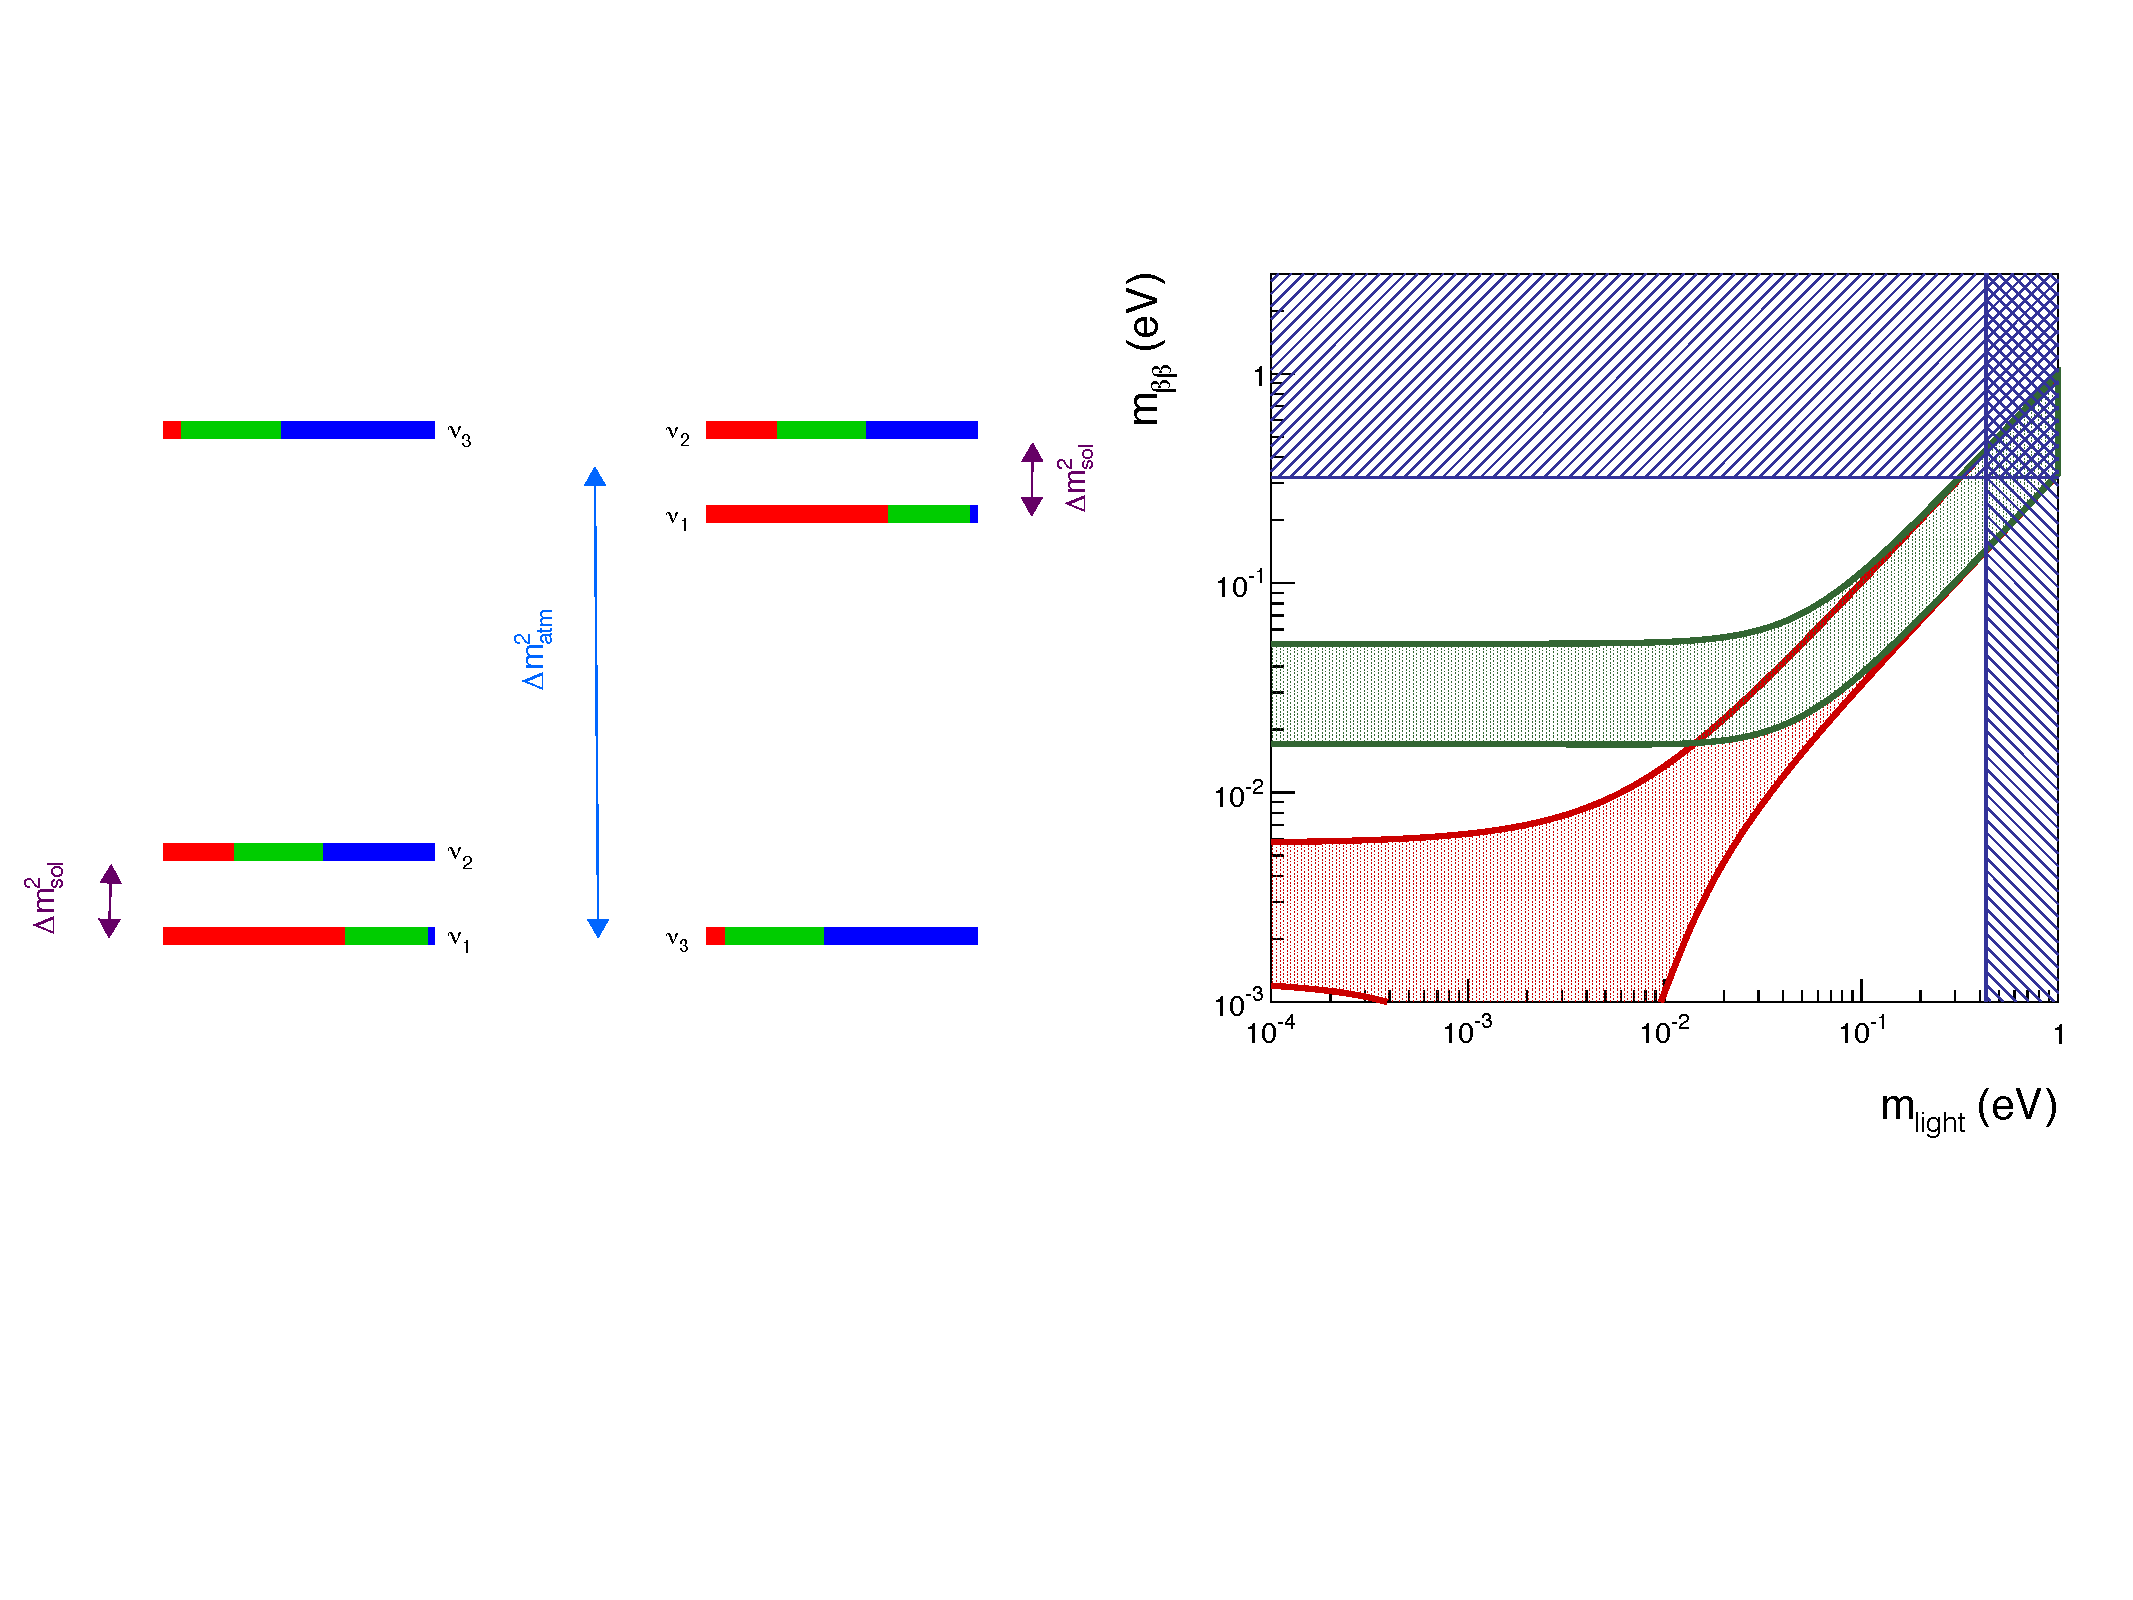
\includegraphics[width=0.99\textwidth]{img/numassmix.pdf}
\caption{\small The left panel shows the normal (left) and inverted (right) mass orderings. The electron, muon and tau flavor content of each neutrino mass eigenstate is shown via the red, green and blue fractions, respectively. The right panel shows the effective neutrino Majorana mass, \mbb, as a function of the lightest neutrino mass, $m_{\rm light}$. The green band corresponds to the inverse hierarchy of neutrino masses, whereas the red corresponds to the normal ordering. The upper bound on the lightest neutrino mass comes from cosmological bounds; the bound on the effective Majorana mass from \bbonu\ constraints.} \label{fig:numass_ordering}
\end{figure}
%%%%%%%%%%

The upper bound on the effective Majorana mass corresponds to the experimental constraint set by the Heidelberg-Moscow (HM) experiment, which was until very recently the most sensitive limit to the half-life of \bbonu: $T^{0\nu}_{1/2}(\GE) \ge 1.9\times10^{25}$ years at 90\% CL.\footcite{KlapdorKleingrothaus:2000sn}  A subgroup of the HM experiment interpreted the data as {\em evidence} of a positive signal, with a best value for the half-life of $1.5\times10^{25}$ years, corresponding to an effective Majorana mass of about 400 meV.\footcite{KlapdorKleingrothaus:2001ke} This claim  was very controversial and still awaits a definitive experimental response.


%%%%%%%%%%%%%%%%%%%%%%%%%%%%%%%%%%%%%%%%%%%%%%%%%%%%%%%%%%
\subsubsection*{Experimental aspects}

The detectors used in double beta decay searches are designed, primarily, to measure the energy of the radiation emitted by a \bb\ source to high precision. In the case of \bbonu, the sum of the kinetic energies of the two released electrons is always the same, and is equal to the mass difference between the parent and the daughter nuclei: $Q_{\bb} \equiv M(Z,A)-M(Z+2,A)$. However, due to the finite energy resolution of any detector, \bbonu\ events are reconstructed within a non-zero energy range centered around \Qbb, typically following a Gaussian distribution. Important backgrounds are those events in the detector of origin not related to \bbonu\ which are reconstructed with energies within this range.

All double beta decay experiments have to deal with an intrinsic background, the standard \bbtnu\ (a SM-allowed process consisting in two simultaneous $\beta$ decays), that can only be suppressed by achieving an energy resolution sufficiently good to separate the continuous spectrum of \bbtnu\ from the Gaussian \bbonu. Backgrounds of cosmogenic origin force the underground operation of the detectors. However, natural radioactivity emanating from the detector materials and surroundings still have the potential to overwhelm the signal peak and hence careful selection of radiopure materials is essential. Additional experimental signatures that allow the distinction of signal and background can further strengthen a result.

Besides energy resolution and control of backgrounds, several other factors such as detection efficiency and the scalability to large masses must be taken into account in the design of a double beta decay experiment. The simultaneous optimization of all these parameters is often challenging, if not impossible, and consequently many different experimental approaches have been proposed. In order to compare them the experimental sensitivity to \mbb is used as a figure of merit:\footcite{GomezCadenas:2010gs}
%%%
\begin{equation}
\mbb = K \ \sqrt{1/\varepsilon} \ \left(\frac{b\cdot\Delta E}{M\cdot t} \right)^{1/4}\, ,
\label{eq:mbb}
\end{equation}
%%%
where $\varepsilon$ is the detection efficiency, $\Delta E$ is the energy resolution window where the \bbonu\ signal will be reconstructed, $b$ is the background rate (in counts per year, kilogram of \bb\ isotope, keV) in the region of interest, $M$ is the \bb\ isotope mass, and $t$ is the data-taking time. 


%%%%%%%%%%%%%%%%%%%%%%%%%%%%%%%%%%%%%%%%%%%%%%%%%%%%%%%%%%
\subsubsection*{The current generation of xenon-based \bbonu\ experiments}
 
 Two xenon-based experiments are currently leading the field: KamLAND-Zen, in which xenon is dissolved in liquid scintillator and EXO-200, a liquid xenon (LXe) TPC. Both have recently published negative results. 
 EXO achieves an energy resolution of 4\% FWHM at \Qbb, and a background rate measured in the \emph{region of interest} (ROI) of $ 4 \times 10^{-3}\ckky$. The total exposure used for the published result is 100 kg$\cdot$year. They have published a limit on the half-life of \bbonu\ of $T_{1/2}^{0\nu}(\XE) > 2 \times 10^{25}$ years.\footcite{Auger:2012ar} 
KamLAND-Zen compensates a worse energy resolution of 10\% FWHM at \Qbb\ with an exposure three times larger, 89.5 kg year. They have published a limit on the half-life of \bbonu\ of $T_{1/2}^{0\nu}(\XE) > 1.9 \times 10^{25}$ years.\footcite{Gando:2012zm} In terms of the effective neutrino mass, the EXO Collaboration quotes a sensitivity ranging between 140 and 380 meV, and KamLAND-Zen quotes a sensitivity ranging between 120 and 250 meV. 


%%%%%%%%%%%%%%%%%%%%%%%%%%%%%%%%%%%%%%%%%%%%%%%%%%%%%%%%%%


%Si el proyecto es continuación de otro previamente financiado, individual o coordinado, deben indicarse con claridad los objetivos y los resultados ya alcanzados de manera que sea posible evaluar el avance real que se propone en el nuevo proyecto. Si el proyecto aborda un tema nuevo, deben indicarse los antecedentes y contribuciones previas de los equipos de investigación que justifiquen su capacidad para llevarlo a cabo.
%
%2. La hipótesis de partida y los objetivos generales perseguidos con el proyecto coordinado en su conjunto, así como la adecuación del proyecto a la Estrategia Española de Ciencia y Tecnología y de Innovación y, en su caso, a Horizonte 2020 o a cualquier otra estrategia nacional  o internacional de I+D+i.
%
%Si la memoria se presenta a la convocatoria de RETOS INVESTIGACIÓN, deberá identificarse el reto cuyo estudio se pretende abordar y la relevancia social o económica prevista.
%
%3. Los objetivos específicos de cada uno de los subproyectos participantes, enumerándolos brevemente, con claridad, precisión y de manera realista (acorde con la duración prevista del proyecto).
%
%En los subproyectos con dos investigadores principales, deberá indicarse expresamente de qué objetivos específicos se hará responsable cada uno de ellos.
%
%4. El detalle de la metodología propuesta en cada uno de los subproyectos participantes, incluyendo la viabilidad metodológica de las tareas. Si fuera necesario, también se incluirá una evaluación crítica de las posibles dificultades de un objetivo específico y un plan de contingencia para resolverlas.
%
%5. La descripción de los medios materiales, infraestructuras y equipamientos singulares a disposición de los participantes que permitan abordar la metodología propuesta.
%
%6. Un cronograma claro y preciso de las fases e hitos previstos en relación con los objetivos planteados en la propuesta en su conjunto.
%
%7. Si se solicita ayuda para la contratación de personal, justificación de su necesidad y descripción de las tareas que vaya a desarrollar.

\subsection{\sc IMPACTO ESPERADO DE LOS RESULTADOS/EXPECTED IMPACT}
\subsection{\sc CAPACIDAD FORMATIVA DEL EQUIPO/TRAINING CAPABILITIES OF THE GROUP}
\subsection{\sc IMPLICACIONES ÉTICAS Y/O DE BIOSEGURIDAD/ETHICS AND SAFETY IMPLICATIONS}

\end{document}

%Los resultados de la fase de R\&D de NEXT (financiada por el CONSOLIDER-INGENIO CUP y con importantes contribuciones de los grupos USA) se han traducido en numerosas publicaciones, presentaciones a congresos y charlas invitada (http://next.ific.uv.es/next/talks.html). NEXT ha sido declarado experimento reconocido del CERN y el comité de física nuclear del DOE norteamericano (NSAC) lo cita como uno de los más interesantes del campo (http://science.energy.gov/~/media/np/nsac/pdf/docs/2014/NLDBD_Report_2014_Final.pdf). 
%
%Así, por ejemplo, la vasija a presión ya ha sido construida y los sensores internos (PMTs y SiPMs) ya han sido adquiridos. También han sido adquiridos 100 kilos de gas xenón enriquecido y 100 kilos de gas xenón empobrecido en \XE.
